\input ../talk-header.tex
\usepackage{centernot}
\usepackage[]{algorithm2e}
\title{Machine Learning}
\subtitle{Neural Networks, part 1}

% If you wish to uncover everything in a step-wise fashion, uncomment
% the following command: 
%\beamerdefaultoverlayspecification{<+->}

\begin{document}

\begin{frame}
  \titlepage
\end{frame}

%%%%%%%%%%%%%%%%%%%%%%%%%%%%%%%%%%%%%%%%%%%%%%%%%%%%%%%%%%%%%%%%%%%%%%
%%%%%%%%%%%%%%%%%%%%%%%%%%%%%%%%%%%%%%%%%%%%%%%%%%%%%%%%%%%%%%%%%%%%%%
%%%%%%%%%%%%%%%%%%%%%%%%%%%%%%%%%%%%%%%%%%%%%%%%%%%%%%%%%%%%%%%%%%%%%%

\talksection{Perceptron}

\begin{frame}{Perceptron}
  \vphrase{Gradient Descent}
\end{frame}

\begin{frame}{Perceptron}
  \begin{itemize}
  \item Supervised
  \item Binary linear classifier
  \item Online learning
  \end{itemize}
\end{frame}

\begin{frame}{Perceptron}
  \only<1>{Beginnings:
    \begin{itemize}
    \item One of first artificial neural networks (ANN's)
    \item Developed in 1957 by Frank Rosenblatt, Cornell University Aeronautical Laboratory
    \item First implemented in software (IBM 704)
    \item Intended to be a machine
    \item Designed for image recognition
    \end{itemize}}
  \only<2>{
    Controversy:
    \begin{itemize}
    \item 1958, press conference, NYT
    \item Rosenblatt too optimistic
    \item 1969, Minsky and Papert
    \end{itemize}
  }
\end{frame}

\begin{frame}{Perceptron}
  \begin{displaymath}
    f(x) = \left\{
      \begin{array}{l l}
        1 & \mbox{if } w\cdot x + b > 0 \\
        0 & \mbox{otherwise}
      \end{array}
      \right.
    \end{displaymath}

    The algorithm terminates if and only if the data is linearly
    separable.
\end{frame}

\begin{frame}{Perceptron}
  \begin{itemize}
  \item Also called ``single-layer perceptron''
  \item Not related to multi-layer perceptron
  \item Feedforward neural network
  \end{itemize}
\end{frame}

\begin{frame}{Perceptron}
  The training data is
  \begin{displaymath}
    \blue{D} = \{(x_1, y_1), \ldots, (x_n, y_n)\}
  \end{displaymath}

  \only<2->{
    \vspace{2mm}
    \blue{$x_{j,i}$} is the value of the $i$th feature of the $j$th training input vector
    
    \blue{$x_{j,0}$} = 1  \hspace{5mm} (the bias is thus $w_0$ rather than $b$)

    \blue{$w_i$} is the weight on the $i$th feature
  }
\end{frame}

\begin{frame}{Perceptron}
  Start by setting the weight vector to zero (or to some small random noise).

  \vspace{5mm}
  For each input vector $j$ in turn:
  \begin{enumerate}
  \item Compute $\hat{y} = f(w\cdot x)$
  \item Update the weights: $w_{i} = w_{i} + (y_j - \hat{y}_j) x_{j,i}$
  \end{enumerate}
\end{frame}

\begin{frame}{Multiclass Perceptron}
  \begin{displaymath}
    \hat{y} = \mbox{argmax}_y f(x, y)\cdot w
  \end{displaymath}

  \begin{displaymath}
    w = w + f(x,y) - f(x,\hat{y})
  \end{displaymath}
\end{frame}

\begin{frame}{Multiclass Perceptron: Example}
  \only<1>{\cimgh{pixels-to-1-class.png}}
  \only<2>{\cimgh{pixels-to-10-classes.png}}
\end{frame}

\begin{frame}{Perceptron History}
  \only<1>{  \begin{itemize}
    \item Perceptron is an example of SPR for image recognition
    \item Initially very promising
    \item IBM 704 \gray{(software implementation of algorithm)}\\[3mm]
    \item Mark 1 Perceptron at the Smithsonian Institution
    \item 400 photocells randomly connected to neurons.
    \item Weights encoded in potentiometers, updated during learning
      by electric motors
    \end{itemize}
    \prevwork{Frank Rosenblatt, The Perceptron: A Probabilistic Model
      for Information Storage and Organization in the Brain, Cornell
      Aeronautical Laboratory, Psychological Review, v65, No. 6,
      pp. 386–-408, 1958. doi:10.1037/h0042519}
  }
  \only<2>{
    \begin{itemize}
    \item Minksy and Papert showed perceptrons are incapable of recognizing
      certain classes of images
    \item AI community mistakenly over-generalized to all NN's
    \item So NN research stagnated for some time\\[3mm]
    \item<2> Single layer perceptrons only recognize linearly separable input
    \item<2> Hidden layers overcome this problem
    \end{itemize}
    \prevwork{M. L. Minsky and S.~A.~Papert, Perceptrons. Cambridge, MA:
      MIT Press. 1969.}
  }
  \only<3>{
    \begin{itemize}
    \item ANN's were slow.
    \item Vanishing gradient problem (Sepp Hochreiter)
    \item Support vector machines (SVN) were faster
    \end{itemize}
  }
  \only<4>{  \begin{itemize}
    \item Inputs = 400 CdS photocells
    \item Weights = potentiometers
    \item Tuning = electric motors
    \end{itemize}}
  \only<5>{\cimghh{mark-1-perceptron.jpg}}
  \only<6>{\cimghhhh{mark-1-perceptron.pdf}
    \prevwork{Frank Rosenblatt, Principles of Neurodynamics: Perceptrons
    and the Theory of Brain Mechanisms, Report No. 1196-G-8, 15 March
    1961, Cornell Aeronautical Laboratory}
  }
\end{frame}

\talksection{Neurons}

\begin{frame}{Inspired by biology}
  \cimghhh{tetanus-neuron.jpg}
  \centerline{\dots but only inspired}
\end{frame}

\begin{frame}
  \frametitle{Linear neuron}
  \begin{displaymath}
    y = b + \sum_i x_i w_i
  \end{displaymath}
  \only<2>{where
    \begin{align*}
      y & = \text{output} \\
      b & = \text{bias} \\
      x_i & = \text{$i^\mathrm{\,th}$ input} \\
      w_i & = \text{weight on $i^\mathrm{\,th}$ input}
    \end{align*}
  }
  \includegraphics<3>[width=.7\textwidth]{linear-neuron.pdf}
\end{frame}

\begin{frame}
  \frametitle{Binary threshold neuron}
  \begin{align*}
    z & = \sum_i x_i w_i \\[2mm]
    y & = \left\{
      \begin{array}{l}
        1  \text{ if } z \ge 0 \\
        0  \text{ otherwise}        
      \end{array}
    \right.
  \end{align*}
  \only<2>{
    where
    \begin{align*}
      z & = \text{total input} \\
      y & = \text{output} \\
      x_i & = \text{$i^\mathrm{\,th}$ input} \\
      w_i & = \text{weight on $i^\mathrm{\,th}$ input}
    \end{align*}
    \prevwork{W. McCulloch and W. Pitts, A logical calculus
      of the ideas immanent in nervous activity. Bulletin of
      Mathematical Biophysics, 7:115--133, 1943.}
  }
  \includegraphics<3>[width=.7\textwidth]{binary-threshold-neuron.pdf}
\end{frame}

\begin{frame}
  \frametitle{Rectified linear neuron}
  \begin{align*}
    z & = b + \sum_i x_i w_i \\[2mm]
    y & = \left\{
      \begin{array}{l}
        z  \text{ if } z \ge 0 \\
        0  \text{ otherwise}        
      \end{array}
    \right.
  \end{align*}
  \only<2>{
    where
    \begin{align*}
      z & = \text{total input} \\
      y & = \text{output} \\
      b & = \text{bias} \\
      x_i & = \text{$i^\mathrm{\,th}$ input} \\
      w_i & = \text{weight on $i^\mathrm{\,th}$ input}
    \end{align*}
  }
  \includegraphics<3>[width=.7\textwidth]{rectified-linear-neuron.pdf}
\end{frame}

\begin{frame}
  \frametitle{Sigmoid neuron}
  \begin{align*}
    z & = b + \sum_i x_i w_i \\[2mm]
    y & = \frac{1}{1+e^{-z}}
  \end{align*}
  \only<2>{
    \blue{(It's differentiable!)}
  }
  \includegraphics<3>[width=.7\textwidth]{sigmoid-neuron.pdf}
\end{frame}

\begin{frame}
  \frametitle{Stochastic binary neuron}
  \begin{align*}
    z & = b + \sum_i x_i w_i \\[2mm]
    p &= \frac{1}{1+e^{-z}} \\[3mm]
    y & = \left\{
      \begin{array}{l}
        1  \text{ with probability } p \\[2mm]
        0  \text{ with probability } 1 - p
      \end{array}
    \right.
  \end{align*}
  \only<2>{\blue{(a probability distribution)}}

  \only<3>{\blue{Can also do something similar with rectified linear
      neurons, produce spikes with probability $p$ with a Poisson
      distribution.}}
\end{frame}

\talksection{Neural Networks}

\begin{frame}{Architecture}
  \only<1>{\vphrase{It's how we connect the dots (the states).}}
  \only<2>{Feedforward neural networks
    \begin{itemize}
    \item Flow is unidirectional
    \item No loops
    \end{itemize}

    \vspace{5mm}
    \blue{Makes linear separators (perceptron).}
  }
  \only<3-4>{\vphrase{Idea: maybe add some layers in the middle}}
  \only<4>{
    What would we put there?

    Maybe choose not to care, call them ``hidden layers''.
  }
\end{frame}

\begin{frame}{Layers}
   Neuron activity at each layer must be a non-linear function of
   previous layer
   
    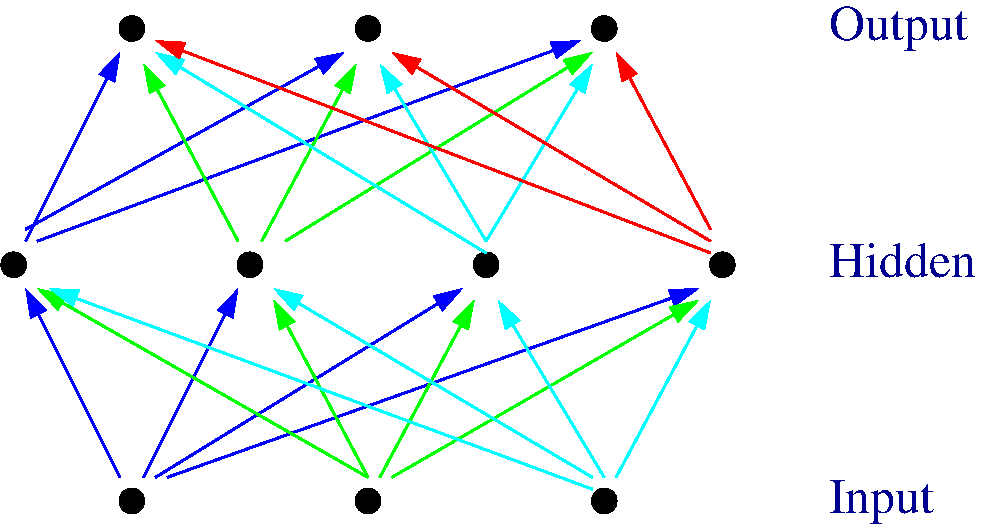
\includegraphics[width=.6\textwidth]{neural-network.pdf}
    
  \red{If more than two hidden layers, then we call it deep}
\end{frame}

\begin{frame}{Recurrent neural networks (RNN)}
  \begin{itemize}
  \item Cycles
  \item Memory
  \item Oscilalations
  \item Harder to train
  \end{itemize}
\end{frame}

\begin{frame}{Recurrent neural networks (RNN)}
\vphrase{Video time}  
\end{frame}

\begin{frame}
  \vphrase{So how would we train such a thing?}
  \only<2>{ It turns
    out that the perceptron algorithm is unstable and prone to many
    problems on deep or non-linear networks.}
\end{frame}

\begin{frame}
  \vphrase{Answer: Backpropagation}
\end{frame}

\begin{frame}
  \cimg{4layers.png}
  \centerline{$(10\times 4) + (4\times 6) + (6\times 8) + (8\times 4) = 144$ connections}
  \prevwork{Shashi Sathyanarayana, A Gentle Introduction to Backpropagation, 22 July 2014.}
\end{frame}

\begin{frame}{}
  \vspace{5mm}
  \blue{\bf Question: How do we find the weights on those 144 connections?}
    
  \only<2-3>{Need a way of refining an initial (random) guess.}
  
  \only<3>{\red{Feedforward is not stable.}}
  \only<4>{\green{So work backwards.}}
\end{frame}

\begin{frame}{Backprogation}
  \begin{itemize}
  \item Modify weights at output layer by an amount proportional to
    the partial-derivative of the error with respect to that weight.
  \item Then do next layer.
  \item Continue through all layers, recomputing partial derivatives at each step.
  \end{itemize}
  
  \only<2>{\blue{Repeat.}}
\end{frame}

\begin{frame}{Backprogation}
  \vphrase{This was hard to learn to do right.}
\end{frame}

\begin{frame}
  \vphrase{Next week: architectures, examples, and code}
\end{frame}


\begin{frame}
  % https://www.pexels.com/photo/man-in-black-jacket-standing-on-black-chair-198747/
  % https://static.pexels.com/photos/198747/pexels-photo-198747.jpeg
  % CC0 license
  \cimgwb{bounce.jpg}
  \vspace{-10.2cm}
  \phrase{questions?\hspace{24mm}}
\end{frame}

\end{document}
